\documentclass[a4paper,12pt]{article}
\usepackage[a4paper,top=1.3cm,bottom=2cm,left=1.5cm,right=1.5cm,marginparwidth=0.75cm]{geometry}
\usepackage{cmap}
\usepackage{mathtext}
\usepackage[T2A]{fontenc}
\usepackage[utf8]{inputenc}
\usepackage[english,russian]{babel}
\usepackage{siunitx}
\usepackage{enumitem}
\usepackage{placeins}

\usepackage{graphicx}
\usepackage{subcaption}
\usepackage{amsmath}
\usepackage{float}

\usepackage{wrapfig}
\usepackage{tabularx}
\usepackage{multirow}
\usepackage{booktabs}

\usepackage{hyperref}
\usepackage[rgb]{xcolor}
\hypersetup{colorlinks=true,urlcolor=blue}
\usepackage{amsmath,amsfonts,amssymb,amsthm,mathtools}
\usepackage{icomma}
\mathtoolsset{showonlyrefs=false}
\usepackage{euscript}
\usepackage{mathrsfs}
\DeclareMathOperator{\sgn}{\mathop{sgn}}
\newcommand*{\hm}[1]{#1\nobreak\discretionary{}
{\hbox{$\mathsurround=0pt #1$}}{}}

\newcommand\labname{Определение петли гистерезиса ферромагнетика магнитооптическим методом}
\newcommand\labnumber{12}

\author{Макаров Лев Евгеньевич}
\title{Лабораторная работа №\labnumber\\\labname}
\date{\today}

\makeatletter
\AddEnumerateCounter{\asbuk}{\russian@asbuk@alph}{щ}
\makeatother

\begin{document}

\begin{titlepage}
    \begin{center}
        {\large МОСКОВСКИЙ ФИЗИКО-ТЕХНИЧЕСКИЙ ИНСТИТУТ (НАЦИОНАЛЬНЫЙ ИССЛЕДОВАТЕЛЬСКИЙ УНИВЕРСИТЕТ)}
    \end{center}
    \begin{center}
        {\large Физтех-школа фотоники, электроники и молекулярной физики}
    \end{center}

    \vspace{4.5cm}
    {\huge
        \begin{center}
            {\bf Отчёт о выполнении лабораторной работы \labnumber}\\
            \labname
        \end{center}
    }
    \vspace{2cm}
    \begin{flushright}
        {\LARGE Автор:\\ Макаров Лев Евгеньевич\\
        \vspace{0.2cm}
        Б04-306}
    \end{flushright}
    \vspace{8cm}
    \begin{center}
        Долгопрудный 2026
    \end{center}
\end{titlepage}

\section{Введение}

\textbf{Цель работы:}
\begin{enumerate}
    \item экспериментально получить петлю гистерезиса ферромагнитного образца магнитооптическим методом;
    \item восстановить зависимость относительной намагниченности от напряжённости магнитного поля;
    \item определить коэрцитивную силу $H_c$ и поле насыщения $H_s$ исследуемого образца.
\end{enumerate}

\textbf{В работе используются:} лазер, исследуемый ферромагнитный образец, катушка, анализатор, фотоприёмник, усилитель, амперметр, резистор, виртуальный осциллограф и источник питания.

\section{Теоретические сведения}

\subsection*{Основные магнитные величины}

В данной работе исследуется петля гистерезиса ферромагнитного образца магнитооптическим методом. Целью работы является получение зависимости намагниченности образца от напряжённости внешнего магнитного поля и определение основных магнитных характеристик: коэрцитивной силы $H_c$ и поля насыщения $H_s$.

Магнитные свойства вещества связаны с наличием магнитных моментов атомов, ионов и электронов. Макроскопической характеристикой магнитного состояния является намагниченность
\[
    \mathbf I = \frac{\sum \mathbf m_i}{V},
\]
где $\mathbf m_i$~--- магнитные моменты частиц, $V$~--- объём образца.

В системе СГС связь между магнитной индукцией $\mathbf B$, напряжённостью магнитного поля $\mathbf H$ и намагниченностью $\mathbf I$ имеет вид
\[
    \mathbf B = \mathbf H + 4\pi \mathbf I.
\]
Для слабомагнитных веществ при малых полях выполняется линейная связь
\[
    \mathbf I = \chi \mathbf H,
\]
где $\chi$~--- магнитная восприимчивость. Тогда
\[
    \mathbf B = \mu \mathbf H, \qquad \mu = 1 + 4\pi\chi.
\]

Диамагнетики имеют отрицательную восприимчивость: $\chi < 0$. Их индуцированный магнитный момент направлен против внешнего поля. Парамагнетики имеют положительную восприимчивость: $\chi > 0$; их магнитные моменты частично ориентируются вдоль внешнего поля, но после выключения поля намагниченность исчезает.

Ферромагнетики обладают спонтанной намагниченностью: ниже температуры Кюри $T_C$ в них возможно упорядоченное состояние магнитных моментов даже при отсутствии внешнего поля. Такое упорядочение объясняется обменным взаимодействием, имеющим квантово-механическую природу. В модели Вейсса его действие описывают молекулярным полем
\[
    H_{\text{мол}} = w I,
\]
где $w$~--- коэффициент молекулярного поля. При $T > T_C$ тепловое движение разрушает ферромагнитное упорядочение, и вещество переходит в парамагнитное состояние.

Реальный ферромагнитный образец обычно разбит на домены~--- области, внутри которых магнитные моменты ориентированы одинаково. Между доменами находятся доменные стенки, где направление намагниченности постепенно меняется. Доменная структура возникает потому, что она уменьшает магнитостатическую энергию образца.

При намагничивании ферромагнетика внешним полем сначала происходит смещение доменных стенок: домены, ориентированные выгодно относительно поля, растут. При больших полях происходит поворот магнитных моментов к направлению поля. Наконец достигается насыщение, когда дальнейшее увеличение поля почти не меняет намагниченность. Соответствующее поле называется полем насыщения $H_s$.

\subsection*{Петля гистерезиса}

Зависимость намагниченности ферромагнетика от внешнего поля неоднозначна и зависит от предыстории образца. При циклическом изменении поля возникает петля гистерезиса. Гистерезис связан с необратимым движением доменных стенок, их закреплением на дефектах и потерями энергии при перемагничивании.

Схематический вид петли гистерезиса показан на рис. \ref{pic:hysteresis}. При увеличении и уменьшении поля значения намагниченности при одном и том же $H$ могут различаться, поэтому зависимость $I(H)$ не является однозначной функцией.

\begin{figure}[H]
    \centering
    
\includegraphics[width=0.5\linewidth]{pictures/1.png}
    \caption{Петля гистерезиса}
    \label{pic:hysteresis}
\end{figure}

Если ферромагнетик довести до насыщения, а затем уменьшить поле до нуля, намагниченность не исчезает. Значение намагниченности при $H=0$ называется остаточной намагниченностью:
\[
    I_r = I(H=0).
\]
Поле противоположного направления, при котором намагниченность обращается в ноль, называется коэрцитивной силой:
\[
    I(H_c)=0.
\]
Чем больше $H_c$, тем труднее перемагнитить материал.

\subsection*{Магнитооптическая регистрация}

В работе петля гистерезиса определяется с помощью эффекта Фарадея. Эффект Фарадея состоит во вращении плоскости поляризации света при прохождении через намагниченное вещество. Угол поворота пропорционален проекции намагниченности на направление распространения света:
\[
    \Psi \sim I_{\parallel}.
\]
Поэтому изменение намагниченности можно регистрировать по изменению интенсивности света после анализатора.

Интенсивность света после анализатора описывается законом Малюса:
\[
    J = J_0 \cos^2\left(\gamma + \Psi_0\sin\omega t\right),
\]
где $J_0$~--- интенсивность падающего света, $\gamma$~--- угол между плоскостью поляризации и осью анализатора, $\Psi_0$~--- амплитуда фарадеевского вращения. При малых углах $\Psi_0 \ll 1$:
\[
    J \approx \frac{J_0}{2}(1+\cos 2\gamma)
    - J_0 \Psi_0 \sin\omega t \sin 2\gamma.
\]
Переменная часть сигнала пропорциональна углу фарадеевского вращения, а значит, и намагниченности образца:
\[
    U_{\text{ф}} \sim \Psi \sim I.
\]
Максимальная чувствительность достигается при $\gamma = 45^\circ$, так как в этом случае $\sin 2\gamma = 1$.

Магнитное поле создаётся катушкой с током. Для используемой установки коэффициент пересчёта равен
\[
    K = 150\ \text{Э/А}.
\]
Следовательно,
\[
    H = Ki.
\]
Ток через катушку определяется по напряжению на последовательно включённом резисторе:
\[
    i = \frac{U_R}{R}.
\]
Отсюда напряжённость магнитного поля выражается через измеряемое напряжение:
\[
    H = K\frac{U_R}{R}.
\]

Таким образом, в эксперименте один сигнал пропорционален магнитному полю $H$, а второй сигнал, снимаемый с фотоприёмника, пропорционален намагниченности $I$. Построение зависимости $I(H)$ даёт петлю гистерезиса. По пересечению петли с осью $I=0$ определяется коэрцитивная сила $H_c$, а по выходу кривой на насыщение определяется поле насыщения $H_s$.

\section{Экспериментальная установка}

В работе используется магнитооптический метод. Магнитное поле создаётся катушкой, внутри которой находится ферромагнитный образец. Изменение намагниченности образца регистрируется по повороту плоскости поляризации света. Схема установки приведена на рис. \ref{pic:setup}.

\begin{figure}[H]
    \centering
    
\includegraphics[width=0.68\textwidth]{pictures/2.png}
    \captionsetup{justification=centering}
    \caption[Блок-схема установки]{
    Блок-схема установки\\
    1 --- лазер, 2 --- образец, 3 --- катушка, 4 --- анализатор, 5 --- фотоприёмник,\\
    6 --- усилитель, 7 --- амперметр,
    8 --- резистор, 9 --- виртуальный осциллограф, 10 --- источник}
    \label{pic:setup}
\end{figure}

Линейно поляризованный свет проходит через исследуемый образец. В магнитном поле из-за эффекта Фарадея плоскость поляризации поворачивается на угол $\psi(t)$, пропорциональный проекции намагниченности образца. После анализатора изменение интенсивности регистрируется фотоприёмником.

Если $\gamma$ --- угол между осью анализатора и исходным направлением поляризации, то по закону Малюса
\begin{equation}
    J(t) = J_0 \cos^2 \left(\gamma + \psi(t)\right).
\end{equation}
При $\gamma \approx 45^\circ$ и малых углах $\psi(t) \ll 1$ изменение интенсивности линейно по $\psi(t)$:
\begin{equation}
    J(t) \approx J_{\text{const}} + A\psi(t).
\end{equation}
Постоянная составляющая при обработке несущественна, поэтому сигнал фотоприёмника можно считать пропорциональным намагниченности:
\begin{equation}
    U_{\text{к1}}(t) \sim \psi(t) \sim I_x(t).
\end{equation}

Напряжённость магнитного поля восстанавливается по сигналу нулевого канала. Поле в катушке пропорционально току:
\begin{equation}
    H_{\text{кат}}(t) = K i(t), \qquad K = 150~\text{Э/А}.
\end{equation}
Ток определяется по напряжению на последовательно включённом резисторе:
\begin{equation}
    i(t) = \frac{U_R(t)}{R}, \qquad U_{\text{к0}}(t) = U_R(t).
\end{equation}
Следовательно,
\begin{equation}
    H_{\text{кат}}(t) = K\frac{U_{\text{к0}}(t)}{R}.
\end{equation}

\section{Результаты измерений и обработка данных}

В ходе работы были зарегистрированы два сигнала: напряжение канала 0, пропорциональное току через катушку, и напряжение канала 1, пропорциональное намагниченности образца. Сначала построим исходную зависимость сигнала фотоприёмника от сигнала катушки. Она показана на рис. \ref{pic:pure}.

\begin{figure}[H]
    \centering
    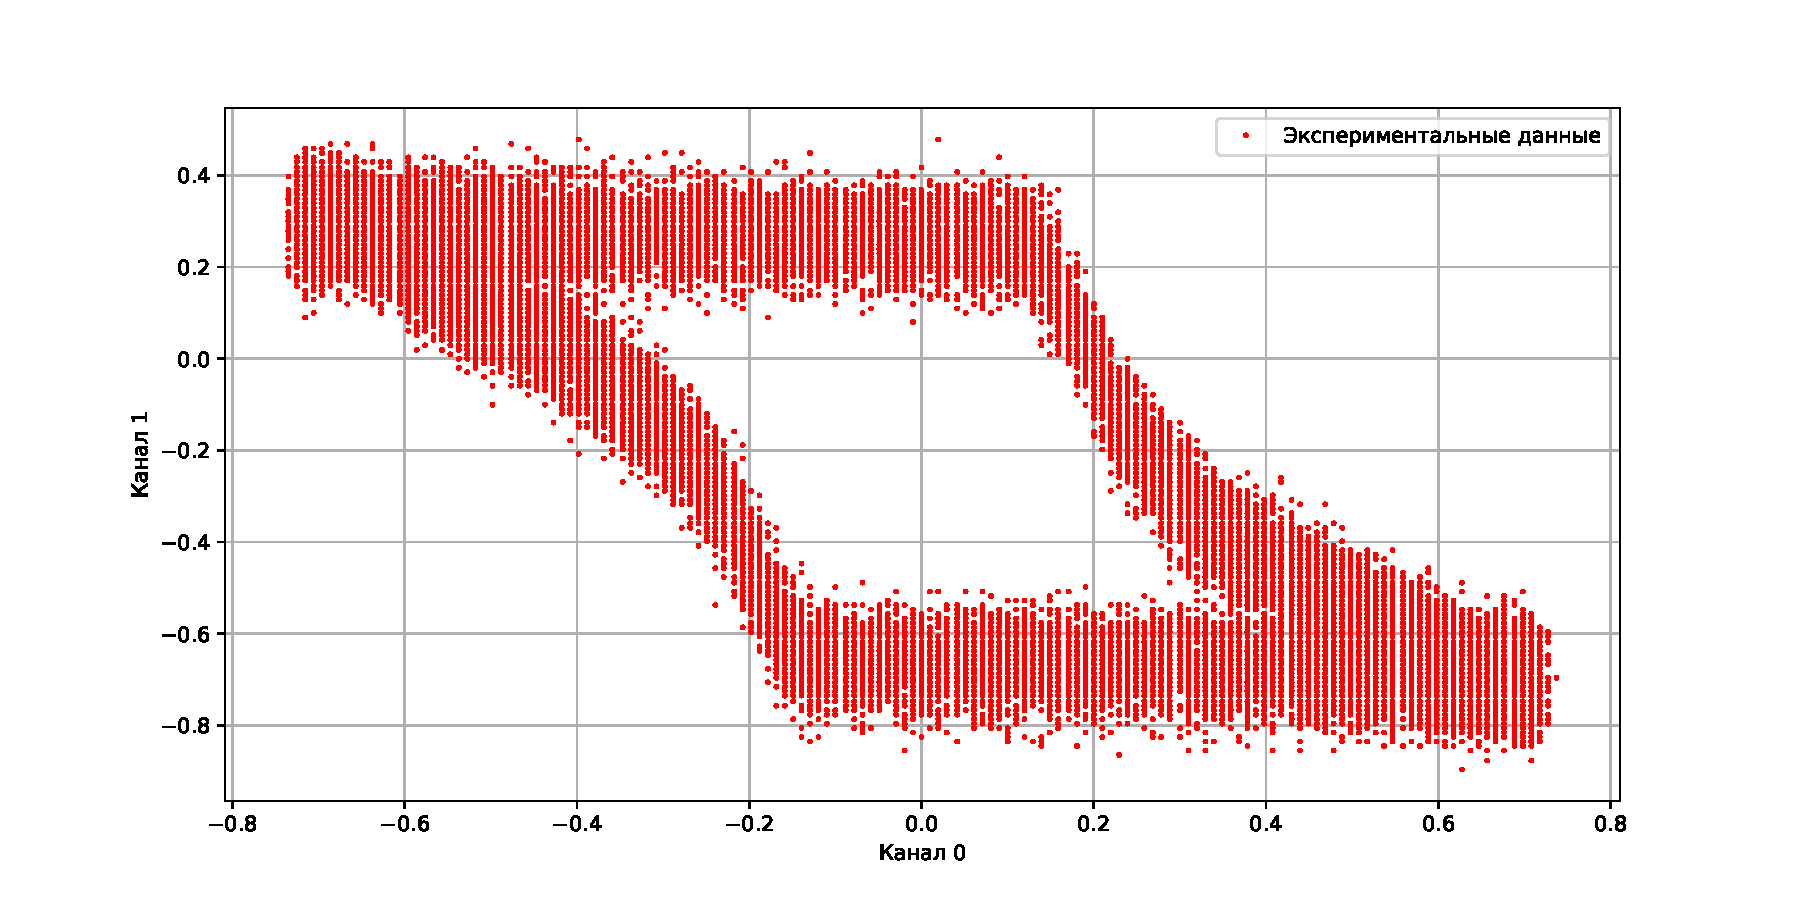
\includegraphics[width=0.92\textwidth]{pictures/graph_pure.pdf}
    \caption{Необработанная зависимость сигнала канала 1 от сигнала канала 0}
    \label{pic:pure}
\end{figure}

Далее сигнал канала 0 был пересчитан в напряжённость магнитного поля $H$, а сигнал канала 1 был нормирован так, чтобы получить относительную намагниченность $I_{\text{отн}}$. Полученная петля гистерезиса приведена на рис. \ref{pic:processed}.

\begin{figure}[H]
    \centering
    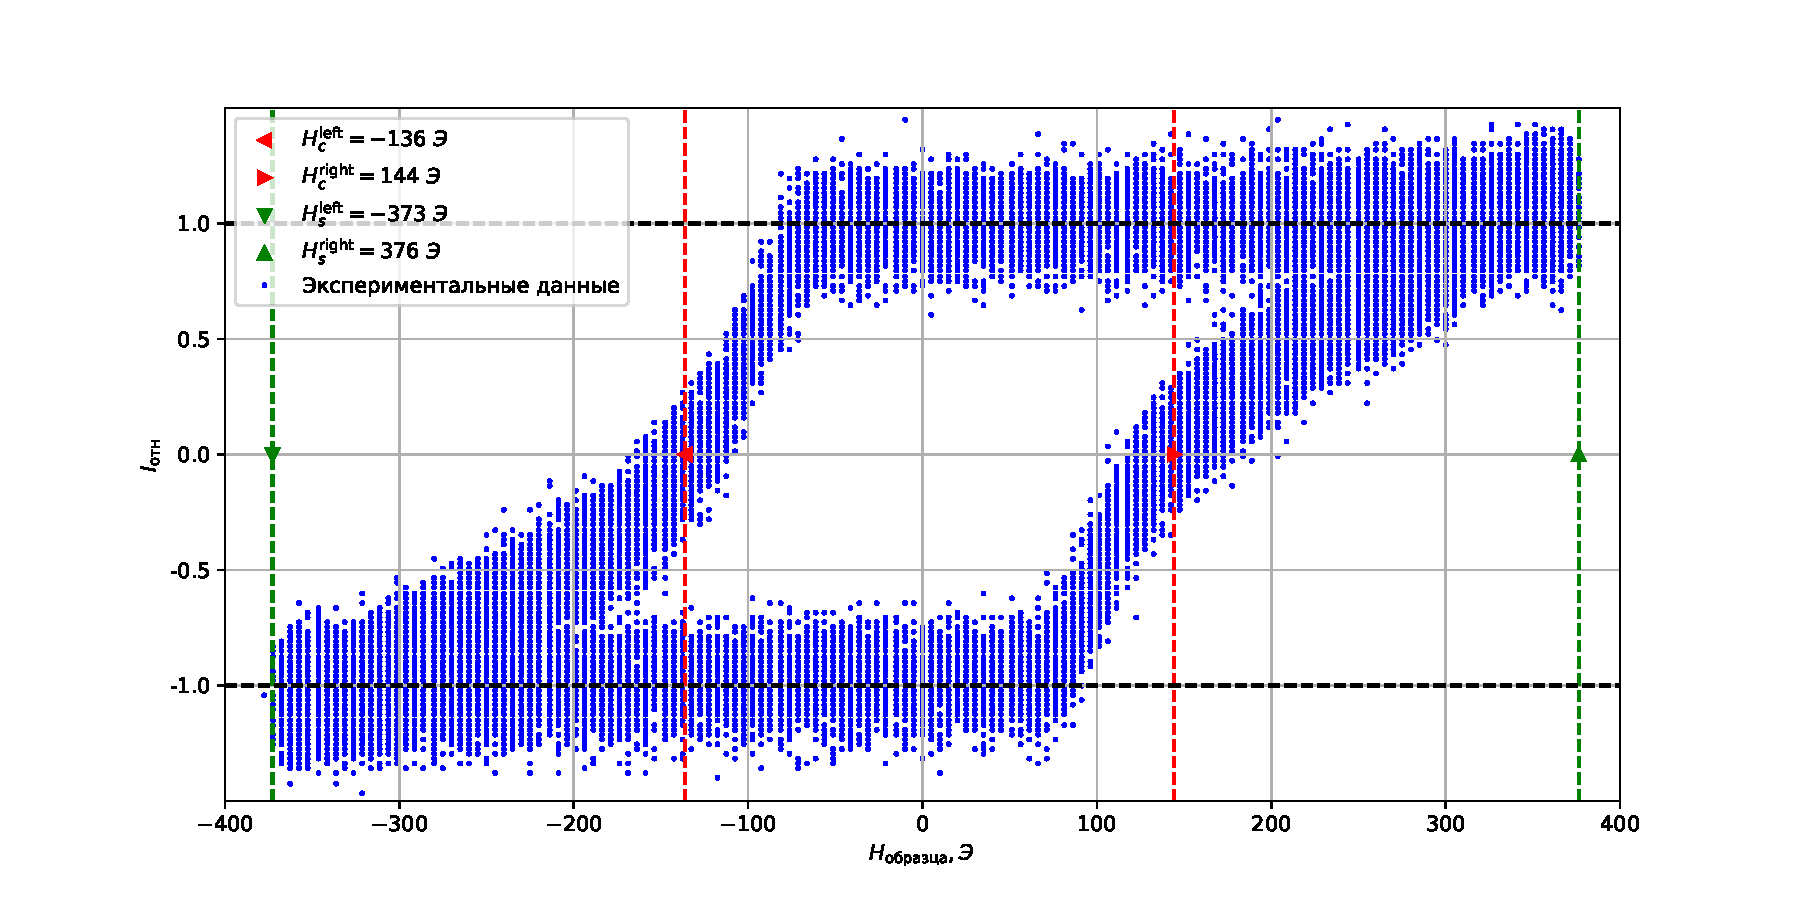
\includegraphics[width=0.92\textwidth]{pictures/graph_I_rel.pdf}
    \caption{Зависимость относительной намагниченности от магнитного поля}
    \label{pic:processed}
\end{figure}

Коэрцитивная сила определялась по точкам пересечения ветвей петли с осью $I_{\text{отн}} = 0$. Так как петля может быть немного сдвинута относительно нуля, использовалось полурасстояние между левым и правым пересечениями:
\begin{equation}
    H_c = \frac{H_c^{\text{right}} - H_c^{\text{left}}}{2}.
\end{equation}

Аналогично поле насыщения находилось как полурасстояние между характерными левым и правым значениями поля насыщения:
\begin{equation}
    H_s = \frac{H_s^{\text{right}} - H_s^{\text{left}}}{2}.
\end{equation}

По обработанной петле гистерезиса получены значения, приведённые в таблице \ref{tab:fields}.

\begin{table}[H]
    \centering
    \caption{Магнитные параметры образца}
    \label{tab:fields}
    \begin{tabular}{cc}
        \toprule
        Величина & Значение \\
        \midrule
        $H_c$ & $140~\text{Э}$ \\
        $H_s$ & $375~\text{Э}$ \\
        \bottomrule
    \end{tabular}
\end{table}

\section{Вывод}

В работе была получена петля гистерезиса ферромагнитного образца магнитооптическим методом. По сигналу фотоприёмника была восстановлена величина, пропорциональная намагниченности, а по напряжению на резисторе --- напряжённость магнитного поля в катушке. По обработанной зависимости $I_{\text{отн}}(H)$ определены основные параметры петли:
\[
    H_c = 140~\text{Э}, \qquad H_s = 375~\text{Э}.
\]
Полученная петля имеет характерный для ферромагнетика вид: при циклическом изменении поля намагниченность зависит от предыстории образца, а при больших по модулю полях выходит на насыщение.

\end{document}
